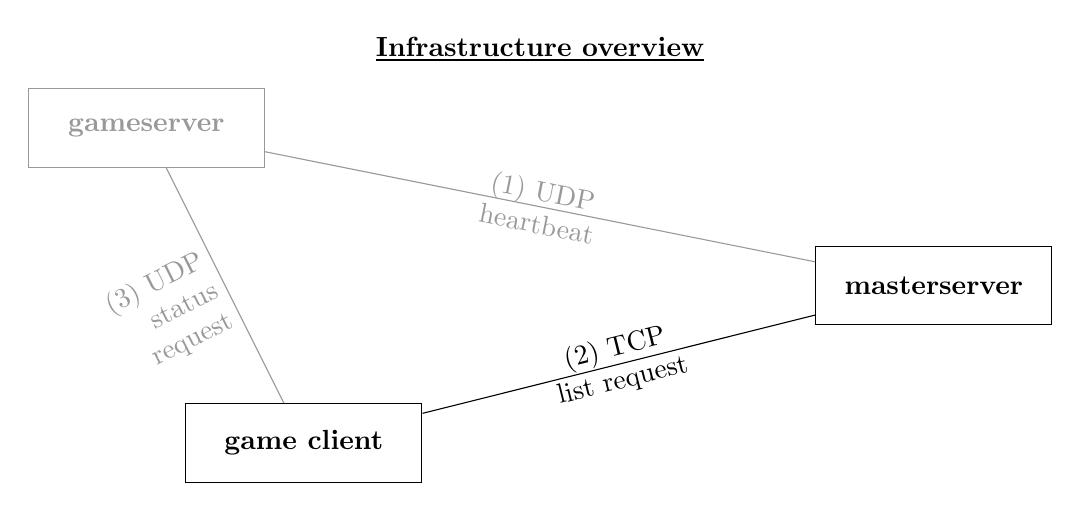
\begin{tikzpicture}

\tikzset{drawbox/.style={draw, rectangle, minimum height=1cm, minimum width=3cm}}
\tikzset{drawline/.style={midway, sloped, text width=2cm, text centered}}

% figure title
\node[rectangle] at (5, 1) (title) {\underline{\bf Infrastructure overview}};

% gameserver, masterserver, game client
\node[drawbox, black!40] at ( 0,  0) (gs) {\bf gameserver};
\node[drawbox] at (10, -2) (ms) {\bf masterserver};
\node[drawbox] at ( 2, -4) (gc) {\bf game client};

% interactions
\draw[black!40] (gs) -- (ms) node[drawline] {(1) UDP\\heartbeat};
\draw (gc) -- (ms) node[drawline] {(2) TCP\\list request};
\draw[black!40] (gc) -- (gs) node[drawline, rotate=90, left, align=right] {(3) UDP\\status request};


\end{tikzpicture}
